\documentclass{article}
\usepackage[utf8x]{inputenc}

\usepackage{xcolor}
% \AddToHook{shipout/before}{%
%   \ifodd\value{page}
%     \pagecolor{blue!10!white}% Odd page colour (light blue)
%   \else
%     \pagecolor{red!10!white}% Even page colour (light red)
%   \fi
% }


\usepackage{geometry}
\geometry{letterpaper, margin=1in}

\providecommand{\tightlist}{%
  \setlength{\itemsep}{0pt}\setlength{\parskip}{0pt}}

\usepackage{adjustbox}
\usepackage[hyphens]{url}
\usepackage{lineno,hyperref}
\modulolinenumbers[5]

%% APA style
\usepackage{graphicx}
\usepackage{caption}

\definecolor{almond}{rgb}{0.94, 0.87, 0.8}
\usepackage{pagecolor}
\usepackage{afterpage}

\begin{document}
\pagestyle{empty}
\thispagestyle{empty}
\pagecolor{gray!30}

\begin{figure}[h]
\begin{adjustbox}{minipage=[c]{\textwidth-10mm},margin= 5mm 15mm 5mm 15mm, frame=1pt, bgcolor=almond,env=center}%
%\begin{adjustbox}{varwidth=\textwidth,bgcolor=almond,margin=3mm {\abovecaptionskip} 3mm 3mm, frame=1pt }
\begin{center}
 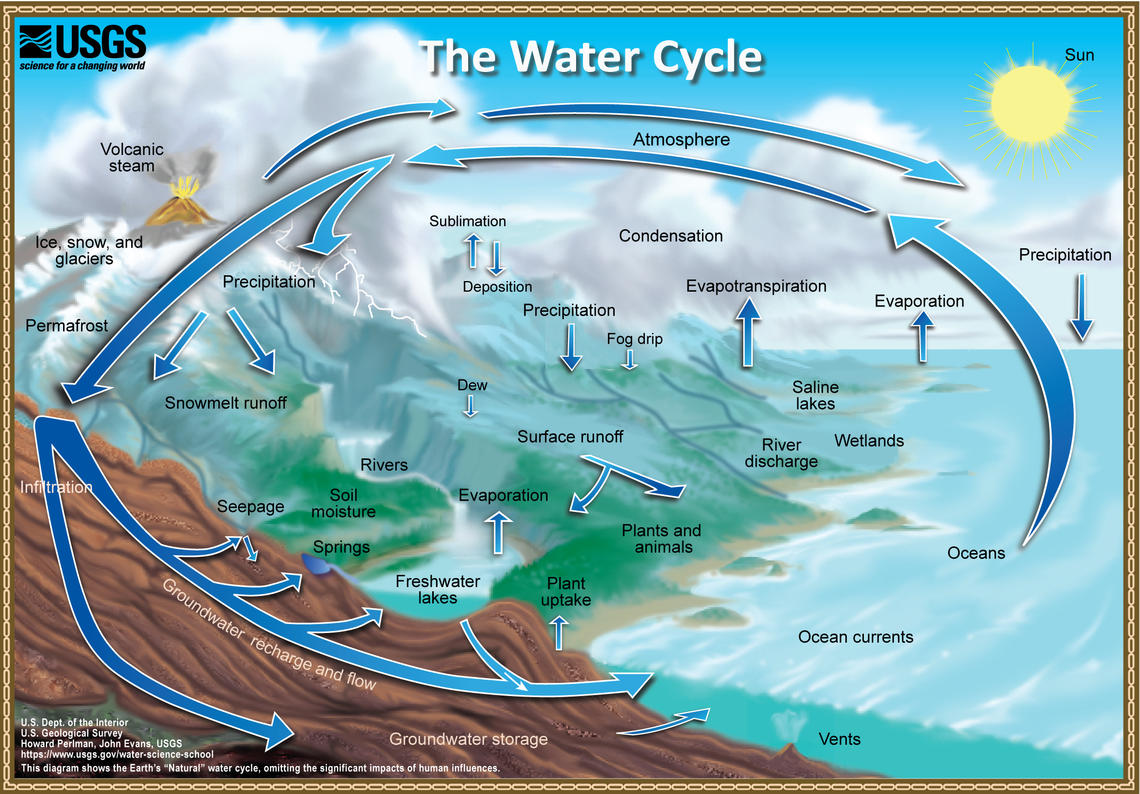
\includegraphics[trim=6mm 6mm 6mm 6mm,clip, width=.6\paperwidth]{image5.jpg}
\end{center}

\begin{center}
\begin{minipage}[t]{0.7\paperwidth}

\medskip
{\huge Open Future Design}
\bigskip

\Large\raggedright
\textbf{Context} People need to coordinate, plan, and maintain cohesion.\newline
\textbf{If} a culture can develop based on shared learning
BUT there is no reliable oracle that can tell us what to expect;\newline
\textbf{Then} use design pattern methods to articulate multiple
futures. This work can be guided by further patterns, e.g.,
to develop languages of:
\medskip

- \emph{future scenarios} → {\sc Participatory Scenario Planning}

\quad\quad cf. {\sc Dérive Comics}, {\sc Meaning Map}, {\sc Reinfuse Expertise} \smallskip

- \emph{roles} → {\sc Play to Anticipate the Future}

\quad\quad cf. {\sc Kaijū Communicator}, {\sc Historian}, {\sc Analyst}, {\sc Designer} \smallskip

- \emph{projects} → {\sc Roadmap}

\quad\quad cf. {\sc Project Action Review}

\end{minipage}
\end{center}
\caption*{Image credit: Howard Perlman, USGS. Public domain.\newline Source:
  \href{https://www.usgs.gov/media/images/water-cycle-natural-water-cycle}{\emph{https://www.usgs.gov/media/images/water-cycle-natural-water-cycle}}}
\end{adjustbox}
\end{figure}



\end{document}